\documentclass{article}
\usepackage[T1]{fontenc}
\usepackage{lmodern}
\usepackage{graphicx}
\usepackage{amsmath,amssymb}
\usepackage[a4paper,margin=2cm]{geometry}
\usepackage[absolute,overlay]{textpos}
\setlength{\TPHorizModule}{1mm}
\setlength{\TPVertModule}{1mm}
\usepackage[indonesian]{babel}
\usepackage{hyperref}
\setlength{\emergencystretch}{2em}
% unit: Halaman 34

\begin{document}

% === Halaman 34 (llm) ===

\vspace{193.05mm}

\begin{itemize}
    \item[\textbf{Legend}] 
    \begin{itemize}
        \item $\bigoplus$ Exclusive-or
        \item $\square$ Addition modulo $2^{32}$
        \item $<<< \text{ Rotation}$
    \end{itemize}
\end{itemize}

% deskripsi: Diagram alur blok kriptografi yang menunjukkan proses enkripsi dari Plaintext (128 bit) menjadi Ciphertext (128 bits), mencakup input whitening, struktur satu ronde dengan S-box, MDS, PHT, rotasi, serta output whitening.
% bbox normalisasi: [0.2100, 0.1400, 0.6300, 0.7900]
\begin{textblock*}{88.20mm}(44.10mm,41.58mm)
\noindent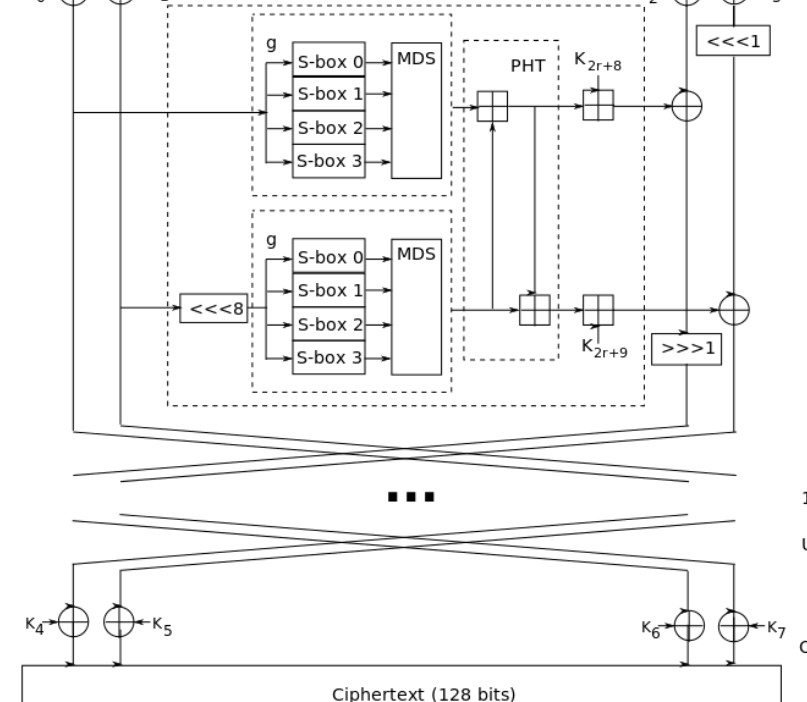
\includegraphics[width=88.20mm,height=193.05mm]{../../images/llm/page_034_img_01.png}%
\end{textblock*}

\end{document}
